\documentclass[x11names,aspectratio=32]{beamer}
\usepackage{ctex}
\usepackage[backend=biber,citestyle=reading]{biblatex}
\usepackage{booktabs}
\usepackage{multirow}
% \usepackage{pgf}
\usepackage{siunitx}

% Theme choice
\usetheme[nofirafonts]{fud}
\usefonttheme{professionalfonts}

\addbibresource{ref.bib}
\graphicspath{{../misc/logo/},{images/}}

\setCJKsansfont[AutoFakeBold,AutoFakeSlant]{KaiTi}


% \pgfdeclareimage[width=.3\linewidth]{titlelogo}{国科大标准Logo横式二(蓝色).png}
% \pgfdeclareimage{footrightlogo}{国科大书法字(白色).png}


\title{Beamer 浅旅}
\author{\href{https://github.com/Memcys/DIY-LaTeX}{Memcys}}
\institute{School of Physical Sciences}
\titlegraphic{%
    
\includegraphics[width=.35\linewidth]{国科大标准Logo横式二(蓝色)}
}
\date{2022-10-02}


\begin{document}
\begin{frame}
    \titlepage
\end{frame}

% ....
% Presentation outline
\begin{frame}{Outline}{概要}
    \tableofcontents
\end{frame}
% ...

% \begin{frame}[fragile]
%     \frametitle{File Structure (Review)}
% \begin{table}
%     \caption[]{Three parts of a typical \TeX source file}
%     \begin{tabular}{lc}
% \verb{
%     \documentclass[]{}
% }
% & Declare the class        
%     \end{tabular}
% \end{table}


% \end{frame}


\section{Lists}
% Lists in beamer (Itemize)
\begin{frame}[fragile,allowframebreaks]{Lists in beamer}{Itemize and enumerate environments}
    \begin{columns}
        \begin{column}{4cm}
            % Itemize:
            \begin{verbatim}
\begin{itemize}
    \item ·
    \item ·
\end{itemize}
\end{verbatim}
            \begin{itemize}
                \item 甲
                \item 乙
                \item 丙
                \item 丁
                \item 戊
            \end{itemize}
        \end{column}

        \begin{column}{.4\textwidth}
            % Enumerate:
            \begin{verbatim}
    \begin{enumerate}
        \item ·
        \item ·
    \end{enumerate}
\end{verbatim}

            \setbeamertemplate{enumerate items}[circle]
            \begin{enumerate}
                \item One
                \item Two
                \item Three
                \item Four
                \item Five
            \end{enumerate}
        \end{column}
    \end{columns}

    \vfill{}

    \begin{columns}

        \begin{column}{.4\textwidth}
            \setbeamertemplate{enumerate items}[square]
            \begin{enumerate}
                \item Eins
                \item Zwei
                \item Drei
                \item Vier
                \item F\"unf
            \end{enumerate}
        \end{column}

        \begin{column}{.4\textwidth}

            \setbeamertemplate{enumerate items}[ball]
            \begin{enumerate}
                \item Un (Une)
                \item Deux
                \item Trois
                \item Quatre
                \item Cinq
            \end{enumerate}

        \end{column}
    \end{columns}

    \vspace{4em}

    \begin{columns}
        \begin{column}{\linewidth}
            % Description:
            \begin{verbatim}
    \begin{description}
        \item[·] ·
        \item[·] ·
    \end{description}
\end{verbatim}

            \begin{description}
                \item[GR] General Relativity
                \item[QM] Quantum Mechanics
                \item[QFT] Quantum Field Theory
                \item[CFT] Conformal Field Theory
            \end{description}
        \end{column}
    \end{columns}
\end{frame}


\section{Tables and Graphs}
% Tables in beamer
\begin{frame}[fragile,allowframebreaks]{Table in beamer}
    % \include{verbatim/table.tex}
    % \scriptsize
    \begin{verbatim}
\begin{table}
    \caption[]{}
    \begin{tabular}{lcr}
        left & center & right \\
        左 & 中 & 右
    \end{tabular}
\end{table}    
    \end{verbatim}

    \vfill{}

    \begin{table}
        \caption{SI base units from \smartcite{NIST-units}. \hyperlink{hyperlink}{\beamerbutton{Click me!}}}
        \label{tb:si-units}
        \begin{tabular}{*{2}{l}c}
            \toprule
            \multirow{2}{*}{Base quantity} & \multicolumn{2}{c}{SI base unit}              \\ \cline{2-3}
                                            & Name                             & Symbol     \\
            \midrule
            length                         & meter                            & \unit{m}   \\
            mass                           & kilogram                         & \unit{kg}  \\
            time                           & second                           & \unit{s}   \\
            electric current               & ampere                           & \unit{A}   \\
            thermodynamic temperature      & kelvin                           & \unit{K}   \\
            amount of substance            & mole                             & \unit{mol} \\
            luminous intensity             & candela                          & \unit{cd}  \\
            \bottomrule
        \end{tabular}
    \end{table}
\end{frame}

\begin{frame}[fragile,allowframebreaks]
    \frametitle{Graphs}
    \scriptsize
    \begin{verbatim}
        \begin{figure}
            \includegraphics[]{}
            \caption[]{}
        \end{figure}
    \end{verbatim}

    \vfill{}

    \begin{figure}
        % \centering
        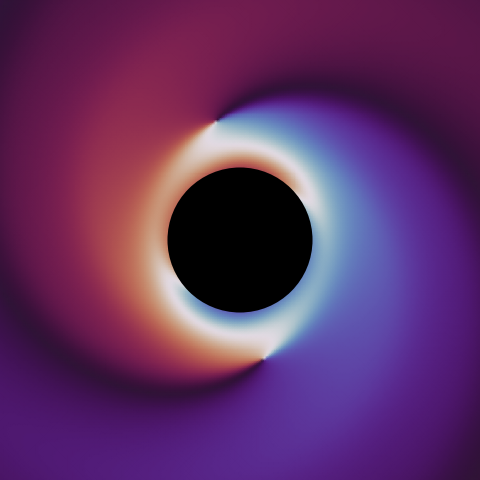
\includegraphics[width=0.18\columnwidth,draft=false]{alpha0p4_phi_phase_1}
        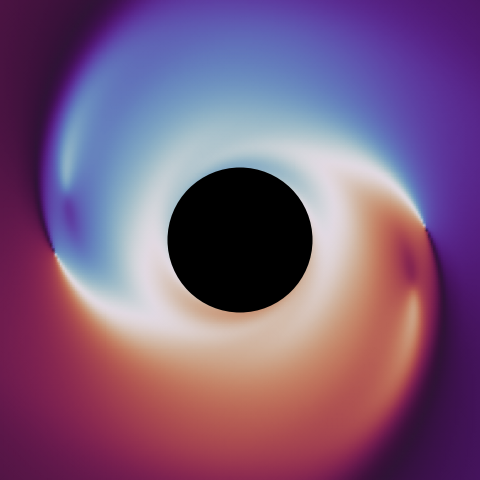
\includegraphics[width=0.18\columnwidth,draft=false]{alpha0p4_phi_phase_2}
        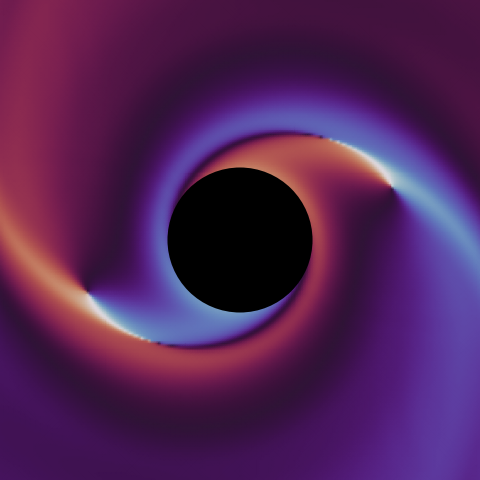
\includegraphics[width=0.18\columnwidth,draft=false]{alpha0p4_phi_phase_3}
        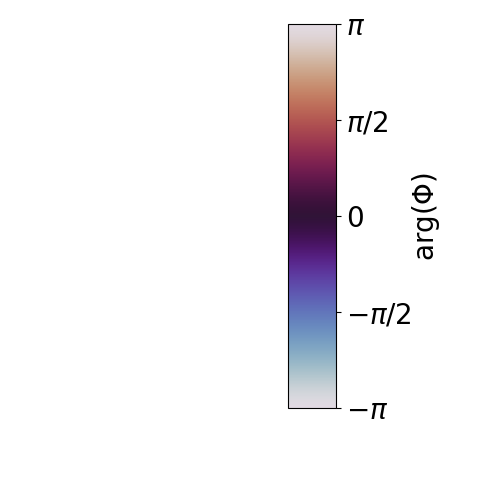
\includegraphics[width=0.075\columnwidth,draft=false,trim=200 0 0 0, clip]{argphi_colorbar}
        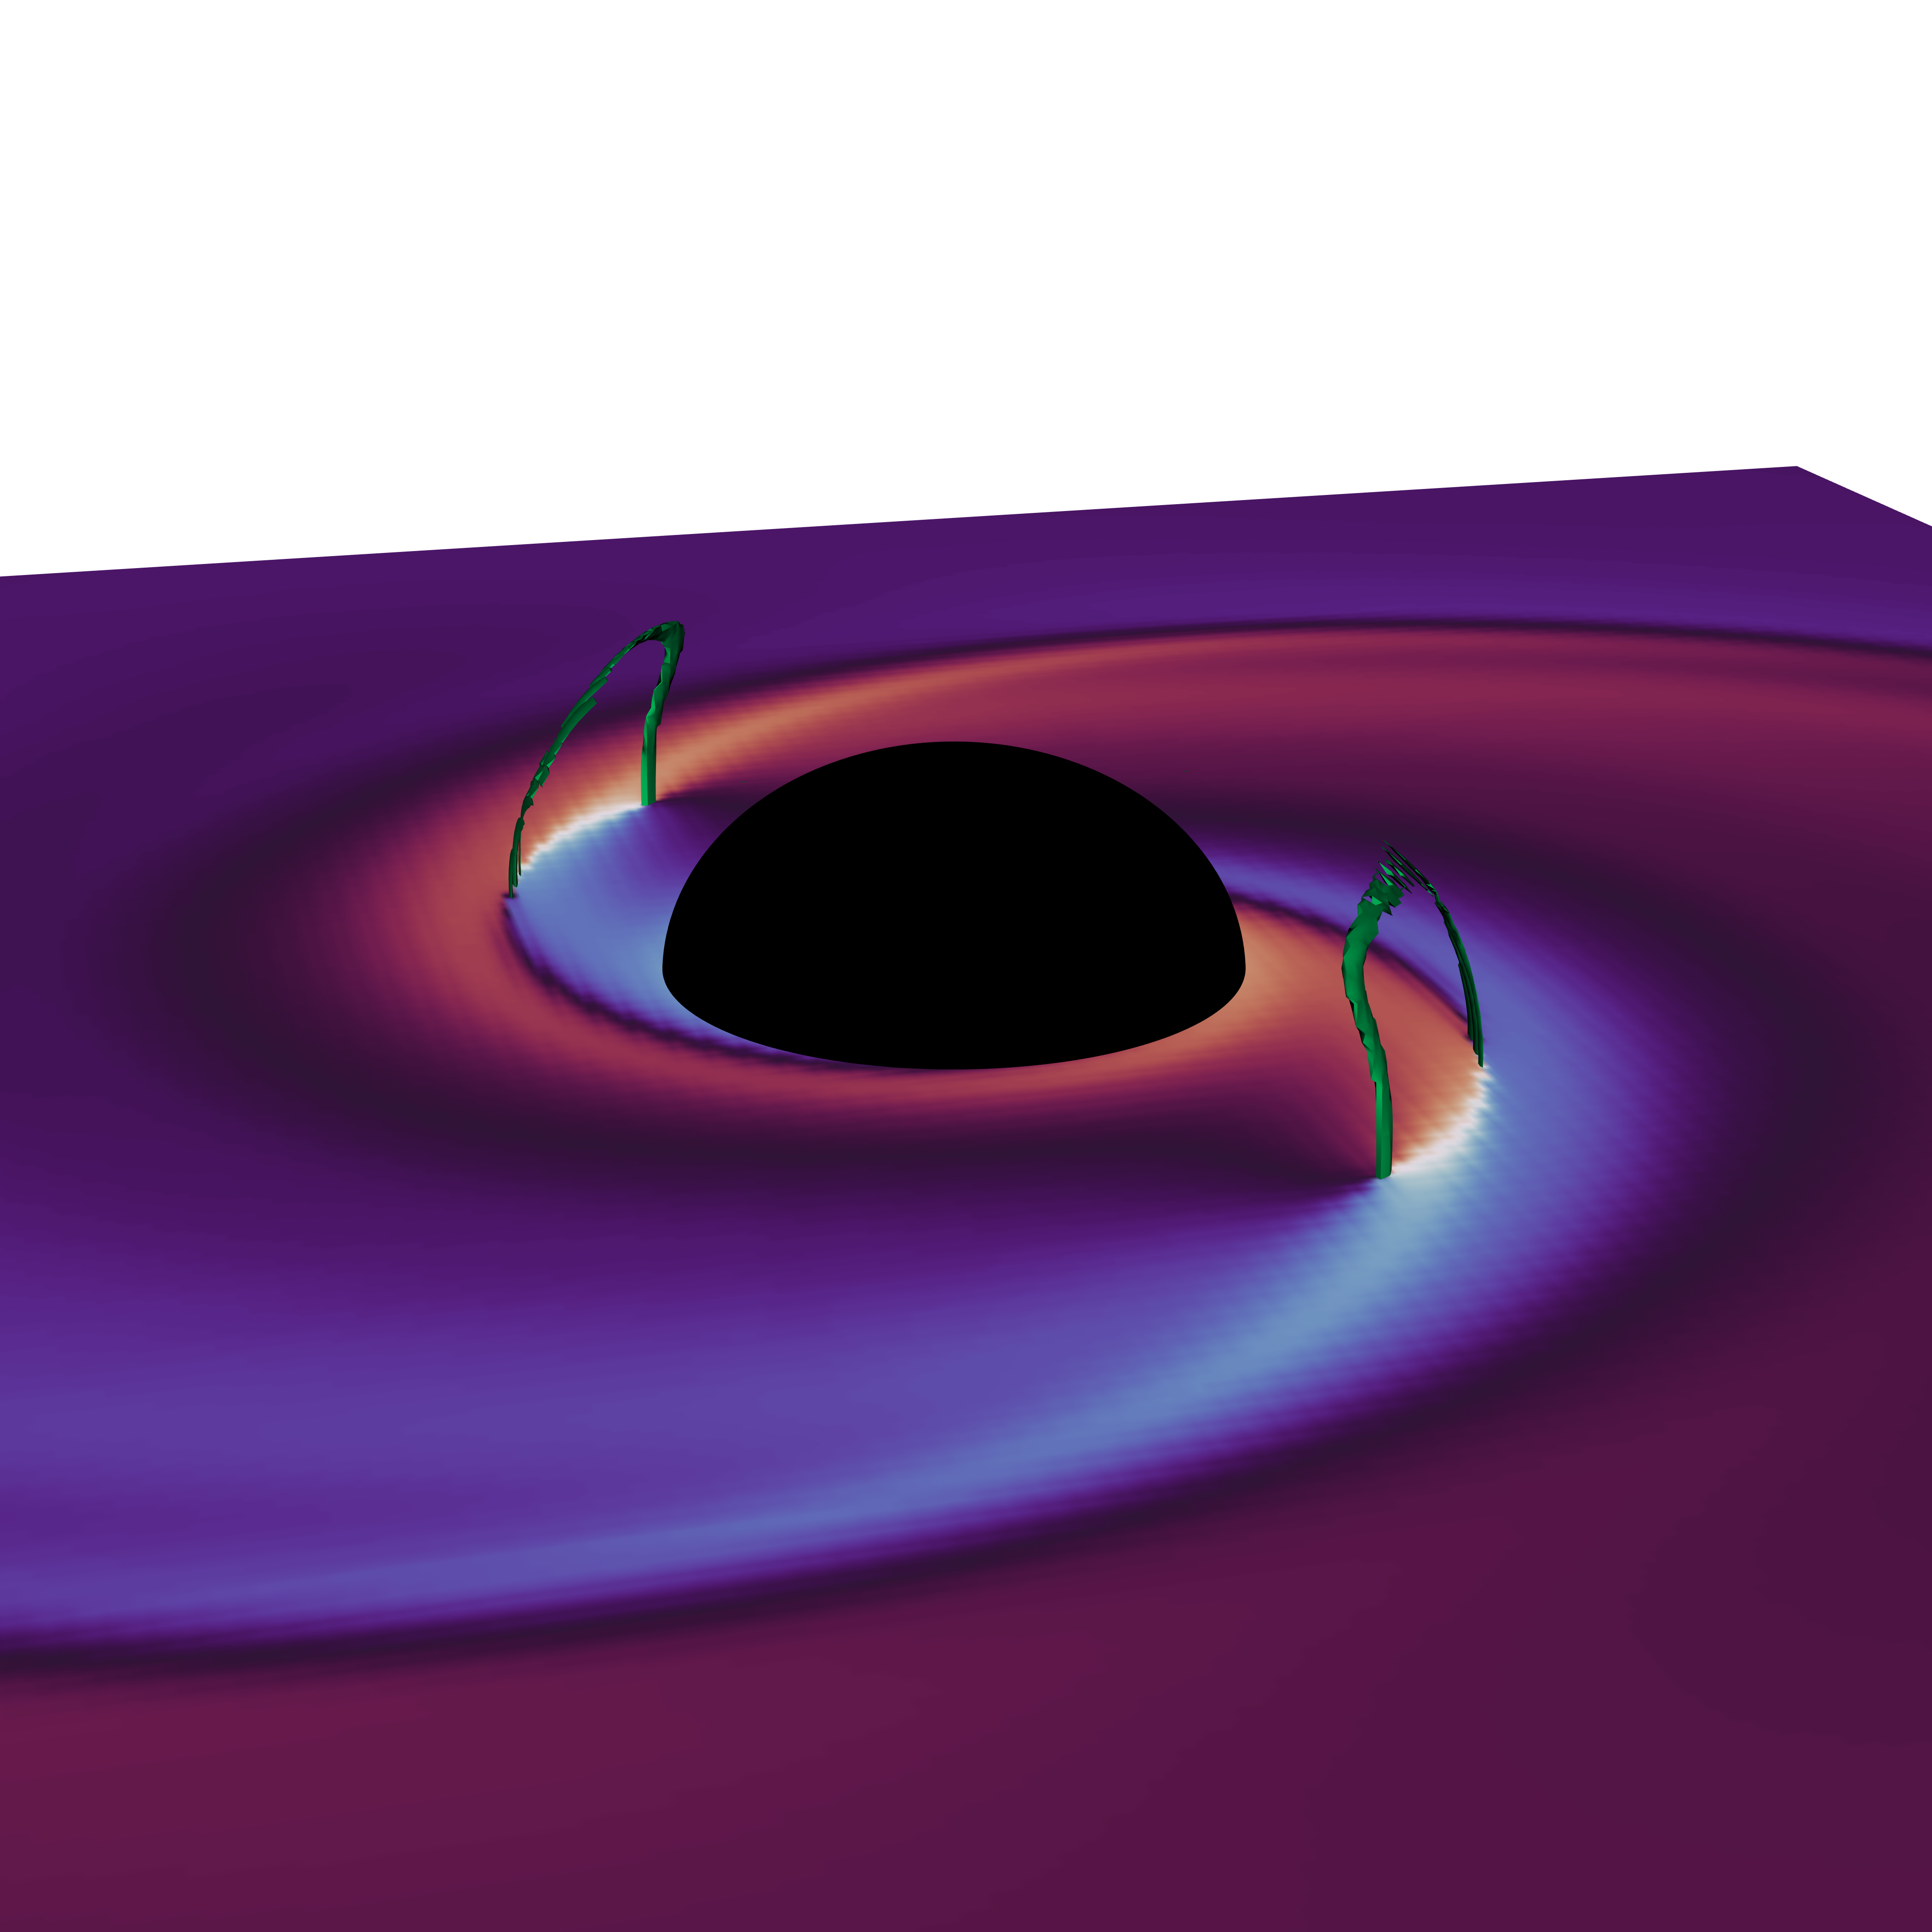
\includegraphics[width=0.18\columnwidth,draft=false]{alpha0p4_phi_3d}

        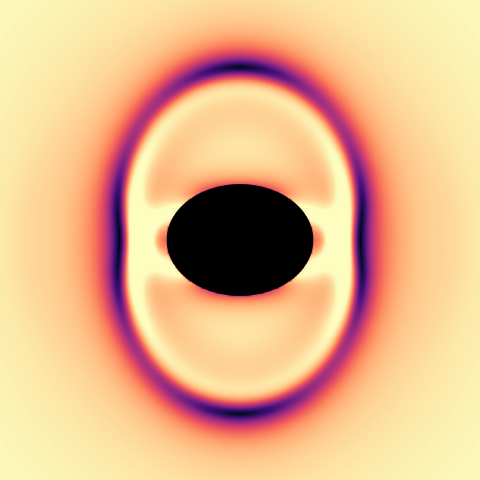
\includegraphics[width=0.18\columnwidth,draft=false]{alpha0p4_phi_mag_1}
        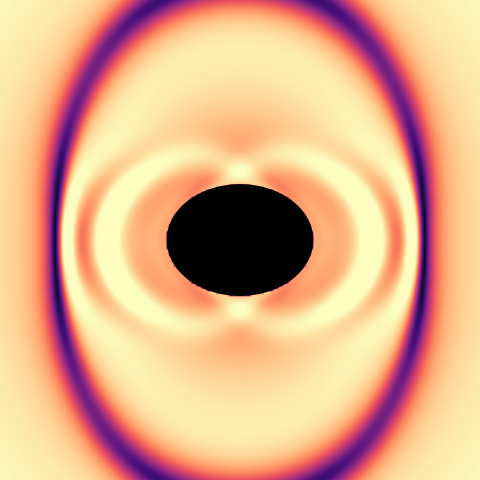
\includegraphics[width=0.18\columnwidth,draft=false]{alpha0p4_phi_mag_2}
        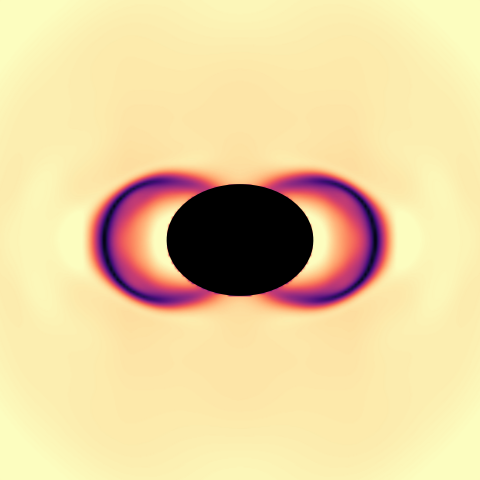
\includegraphics[width=0.18\columnwidth,draft=false]{alpha0p4_phi_mag_3}
        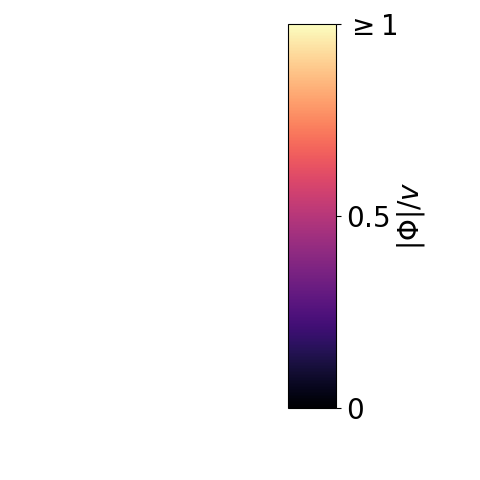
\includegraphics[width=0.078\columnwidth,draft=false,trim=200 0 0 0, clip]{magphi_colorbar}
        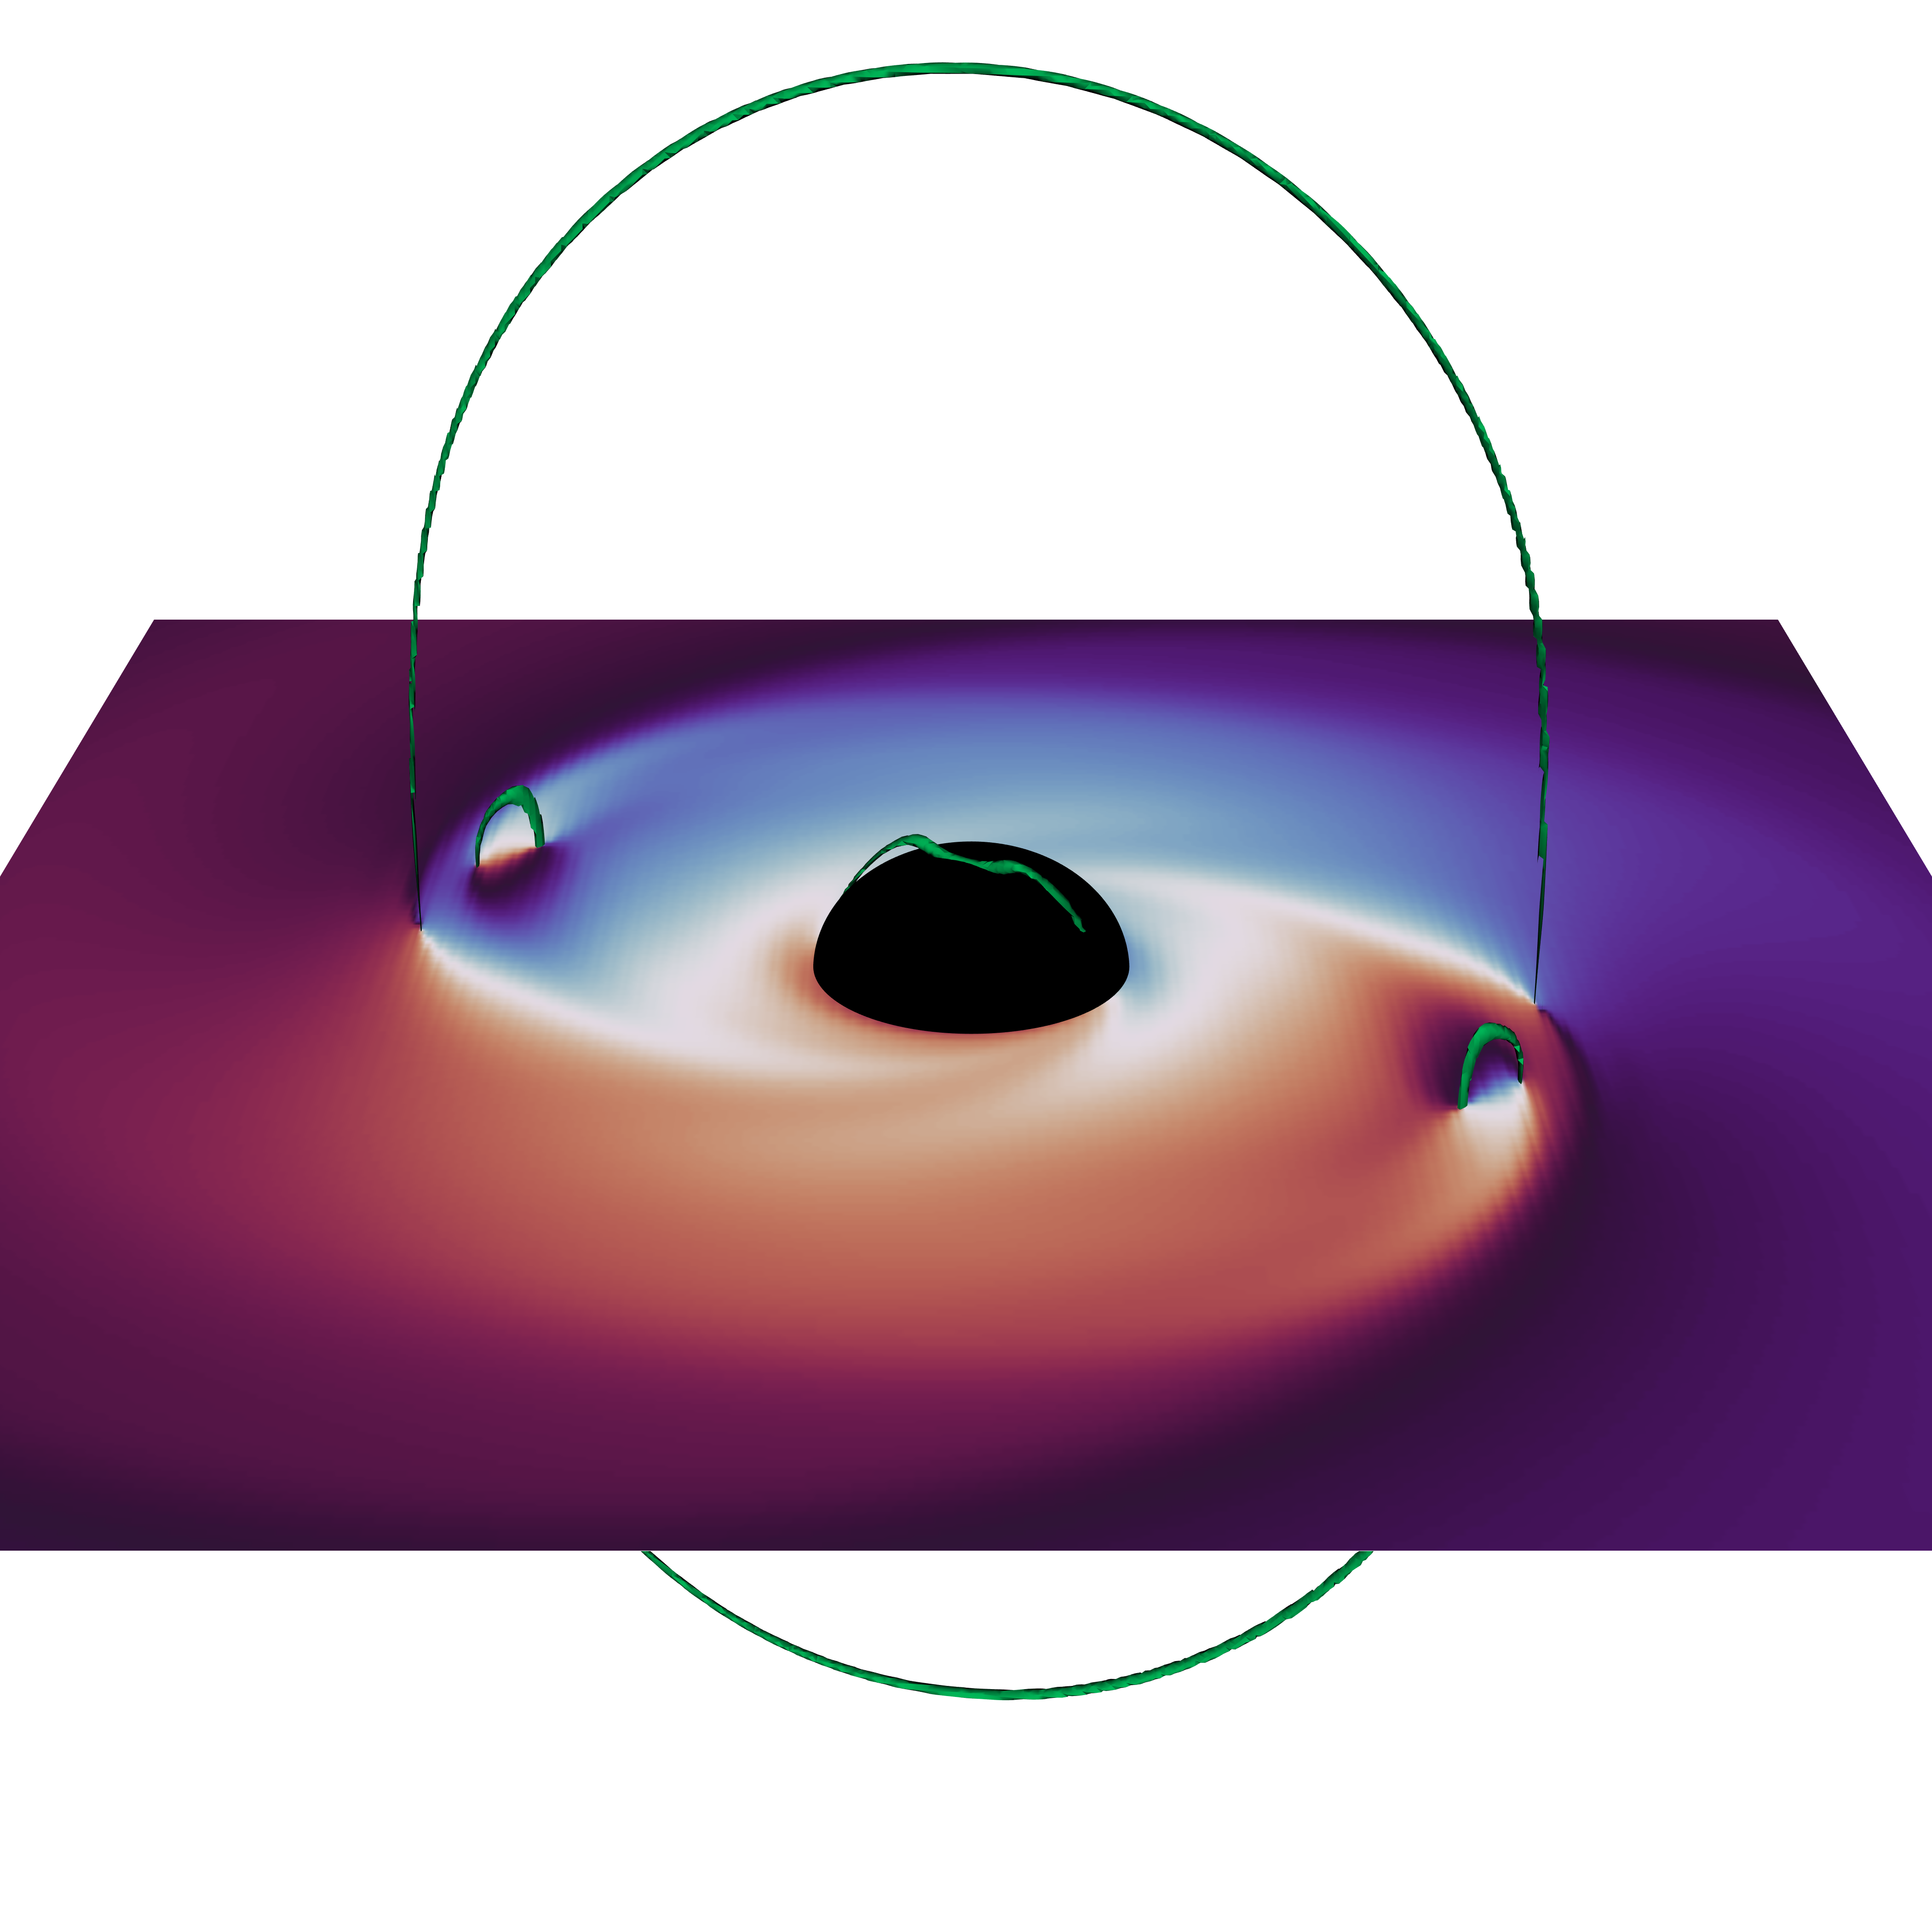
\includegraphics[width=0.18\columnwidth,draft=false]{alpha0p3_phi_3d}
        \caption{Graphs from \smartcite{East2022}.}
    \end{figure}
\end{frame}


\section{Blocks}
% Blocks in beamer
\begin{frame}[fragile]{Blocks in beamer}{}
    \begin{columns}
    \begin{column}{.27\textwidth}
        \begin{verbatim}
\begin{block}{}
\end{block}
        \end{verbatim}
    \end{column}
    \begin{column}{.35\textwidth}
        \begin{verbatim}
\begin{alertblock}{}
\end{alertblock}
        \end{verbatim}
    \end{column}
    \begin{column}{.35\textwidth}
        \begin{verbatim}
\begin{exampleblock}{}
\end{exampleblock}
        \end{verbatim}
    \end{column}
\end{columns}

    \begin{block}{Block 1}
        This is a simple block in beamer.
    \end{block}

    \begin{alertblock}{Block 2}
        This is an alert block in beamer.
    \end{alertblock}

    \begin{exampleblock}{Block 3}
        This is an example block in beamer.
    \end{exampleblock}
\end{frame}

% Blocks in beamer
\begin{frame}[fragile]{Math related blocks in Beamer}{Theorem, Corollary and Proof}
    \begin{columns}
    \begin{column}{.3\textwidth}
        \begin{verbatim}
\begin{theorem}
\end{theorem}
\end{verbatim}
    \end{column}
    \begin{column}{.35\textwidth}
        \begin{verbatim}
\begin{corollary}
\end{corollary}
\end{verbatim}
    \end{column}
    \begin{column}{.3\textwidth}
        \begin{verbatim}
\begin{proof}
\end{proof}
        \end{verbatim}
    \end{column}
\end{columns}

    \begin{theorem}[Relativity Principle]
        The laws of physics take an identical form in all inertial systems.
    \end{theorem}

    \begin{corollary}
        Lorentz (Poincar\'e) invariance.
    \end{corollary}

    \begin{proof}
        Checked by experiments.
    \end{proof}

\end{frame}

\section{Citations, Footnotes and Hyperlinks}
\begin{frame}[fragile]
    \frametitle{Citations, footnotes \& hyperlinks}
    \begin{verbatim}
\cite{}
\footnote{}
\hyperlink{}{}
\end{verbatim}

    本文档参考 \smartcite{beamer-web} 中 \href{https://latex-beamer.com/quick-start/}{LaTeX Beamer introduction / Quick-start guide} 和 \href{https://latex-beamer.com/tutorials/environments/}{8 Beamer Environments you Should be Familiar With} 以及 \footnote{若已安装 TeXLive 完整包,通过 texdoc beamer 即可查看 \cite{beamer-doc}} \emph{Beamer User Guide}\smartcite{beamer-doc}

    \verb|\hyperlink|
    可以实现不同页面的跳转\label{hyperlink},例如 \hyperlink{tb:si-units}{\beamerbutton{SI base units}}


\end{frame}


\section{Beamer Themes}
\begin{frame}[fragile]
    \frametitle{Use a beamer theme}
    \begin{verbatim}
\usetheme{}
\usecolortheme{}
\usefonttheme[]{}
\end{verbatim}

    常用的主题可以在 \href{https://hartwork.org/beamer-theme-matrix}{Beamer Theme Matrix} 中方便预览

    本文档使用了基于 \href{https://github.com/elauksap/focus-beamertheme}{focus} 主题修改定制的 \href{https://github.com/Memcys/fud-beamertheme}{fud} 主题
\end{frame}

\section{Workflow}
\begin{frame}
    \frametitle{Creating a Beamer Presentation}
    \begin{enumerate}
        \item Setup the files (one folder for each presentation)
        \item Structure the presentation (create (sub-)sections)
        \item Create a PDF file (with an outline)
        \item Create frames
        \item Test the presentation
        \item Create a handout
    \end{enumerate}

\end{frame}


% \section{References}
\begin{frame}
    \frametitle{References}
    % \nocite{*}
    \small
    \printbibliography


\end{frame}


\begin{frame}[focus]
    Thanks to your attendance
\end{frame}

\end{document}